\subsection{PAH intensities}
\label{sect:pah_ratios}

Both the 6.2 and 7.7~$\mu$m features are thought to be coming from ionized PAHs and the 11.3~$\mu$m feature from neutral PAHs. Therefore we expect to see a correlation between the intensities of 6.2 and 7.7~$\mu$m PAH features normalized by the 11.3~$\mu$m feature. In Figure \ref{PAHlines} we compare the PAH flux ratios of 7.7/11.3  and 6.2/11.3 features. The figure shows a good correlation between these two PAH line ratios, consistent with that of the SINGS sample shown by \citet{Smith:2007lr}.
A similar correlation was also reported by  \citet{Galliano2008} for a sample of galaxies and a handful of extended H{\sc ii} regions
and by \citet{Vermeij2002} for Galactic and Magellanic Cloud {\sc ii}regions. This provides evidence that the PAH emission from M31 is not unusual. 

%SPW: Fig 10 should mention what's in the "SINGS sample." �Whole galaxies? Central regions? �What?
\begin{figure}
\centering
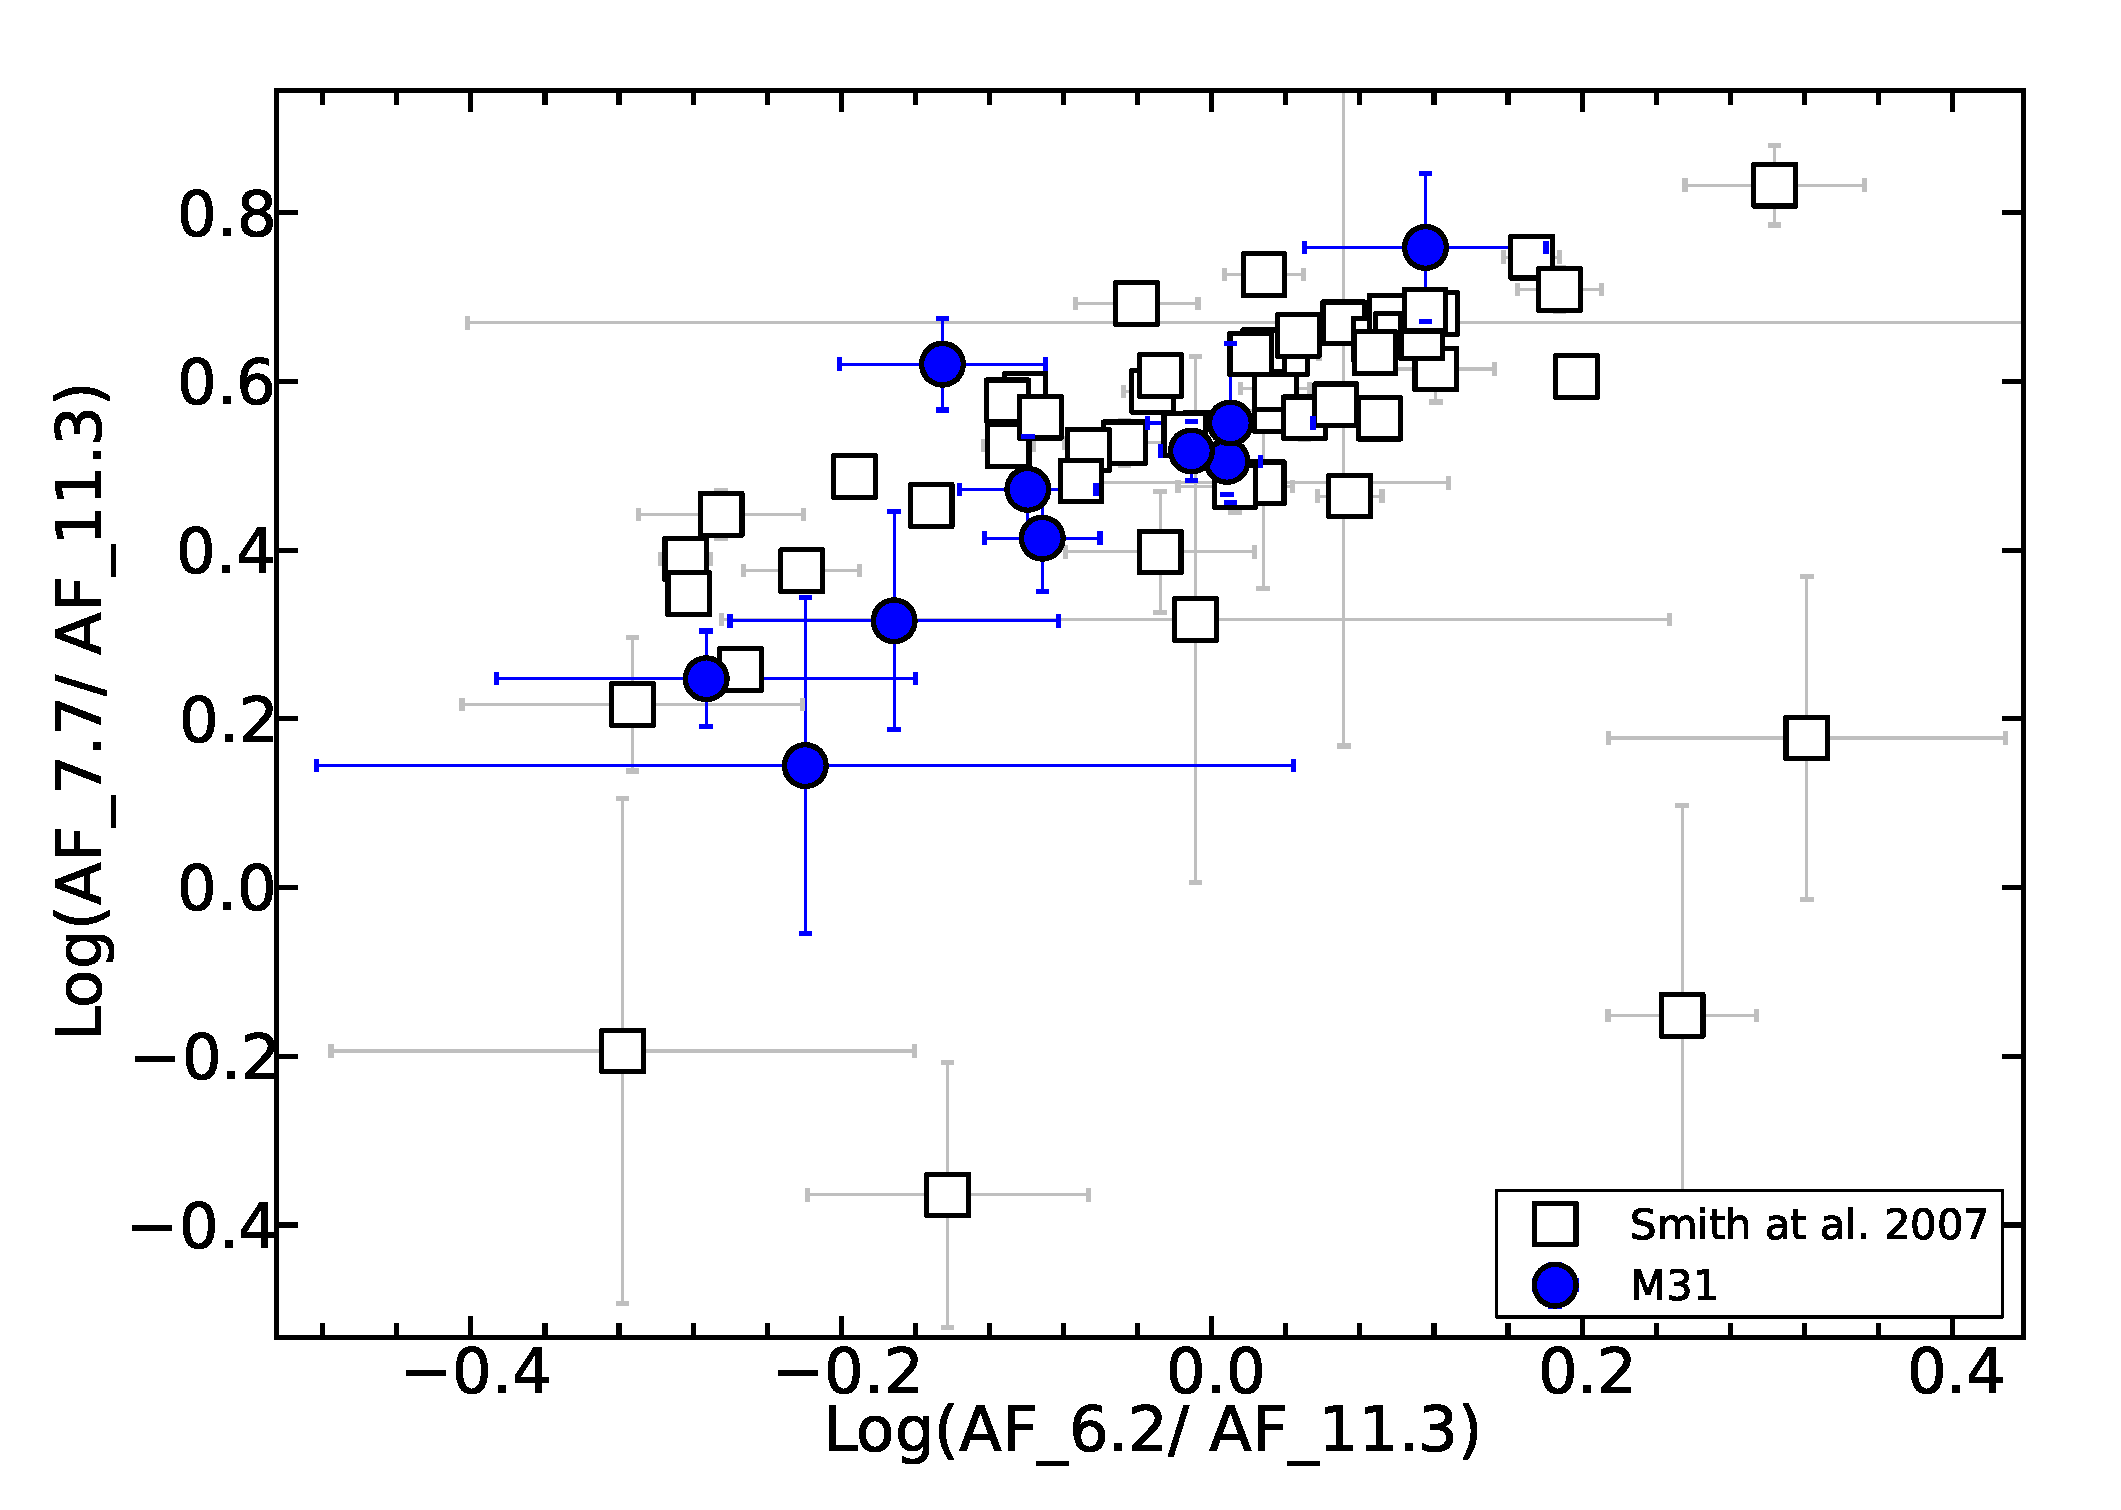
\includegraphics[scale = 0.25]{./SINGSnMy.eps}
\caption{Ratios of PAH feature fluxes (7.7~$\mu$m/11.3~$\mu$m versus 6.2~$\mu$m/11.3~$\mu$m) for 10 regions in M31.
Open squares represent the SINGs sample from \citet{Smith:2007lr}.
}
\label{PAHlines}
\end{figure}

\subsection{PAH equivalent widths versus radiation hardness}
\label{sect:eqw_rh}


\begin{figure}
\centering
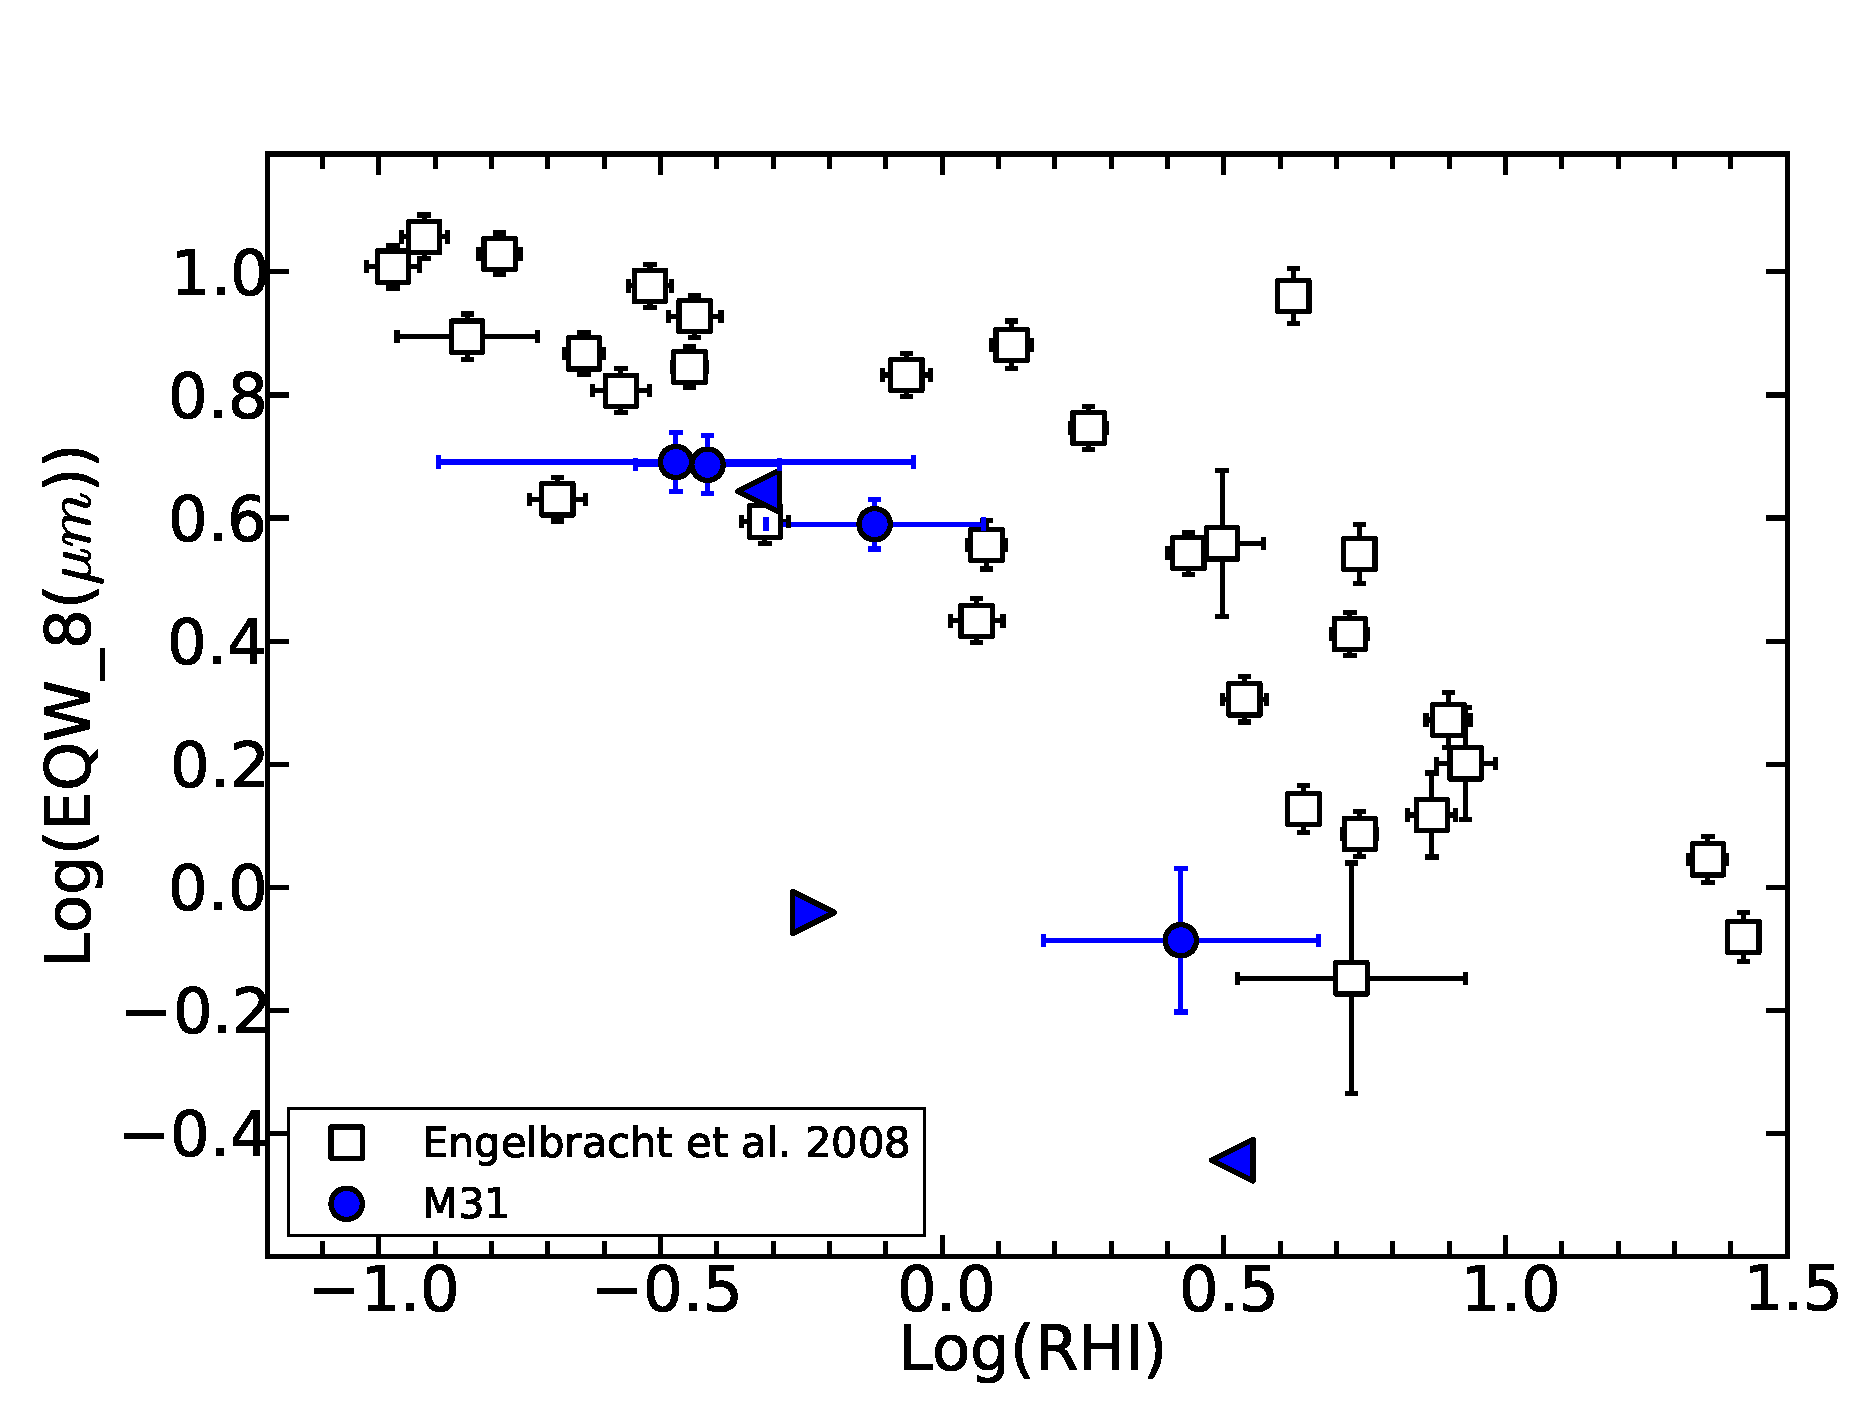
\includegraphics[scale=0.25]{./englvsmy.eps}
\caption{Equivalent width of the 8~$\mu$m PAH feature versus radiation hardness index (RHI) for the M31 sample (blue). 
The 8$\mu$m feature is a combination of the 7.7, 8.3 and 8.6~$\mu$m PAHFIT components. 
Open squares represent the starburst galaxy sample from \citet{Engelbracht_2008}. 
For M31 spectra with undetected lines, triangles represent upper (left-pointing triangles) and lower (right-pointing triangles) limits.}
\label{englII}
\end{figure}

\begin{figure}
\centering
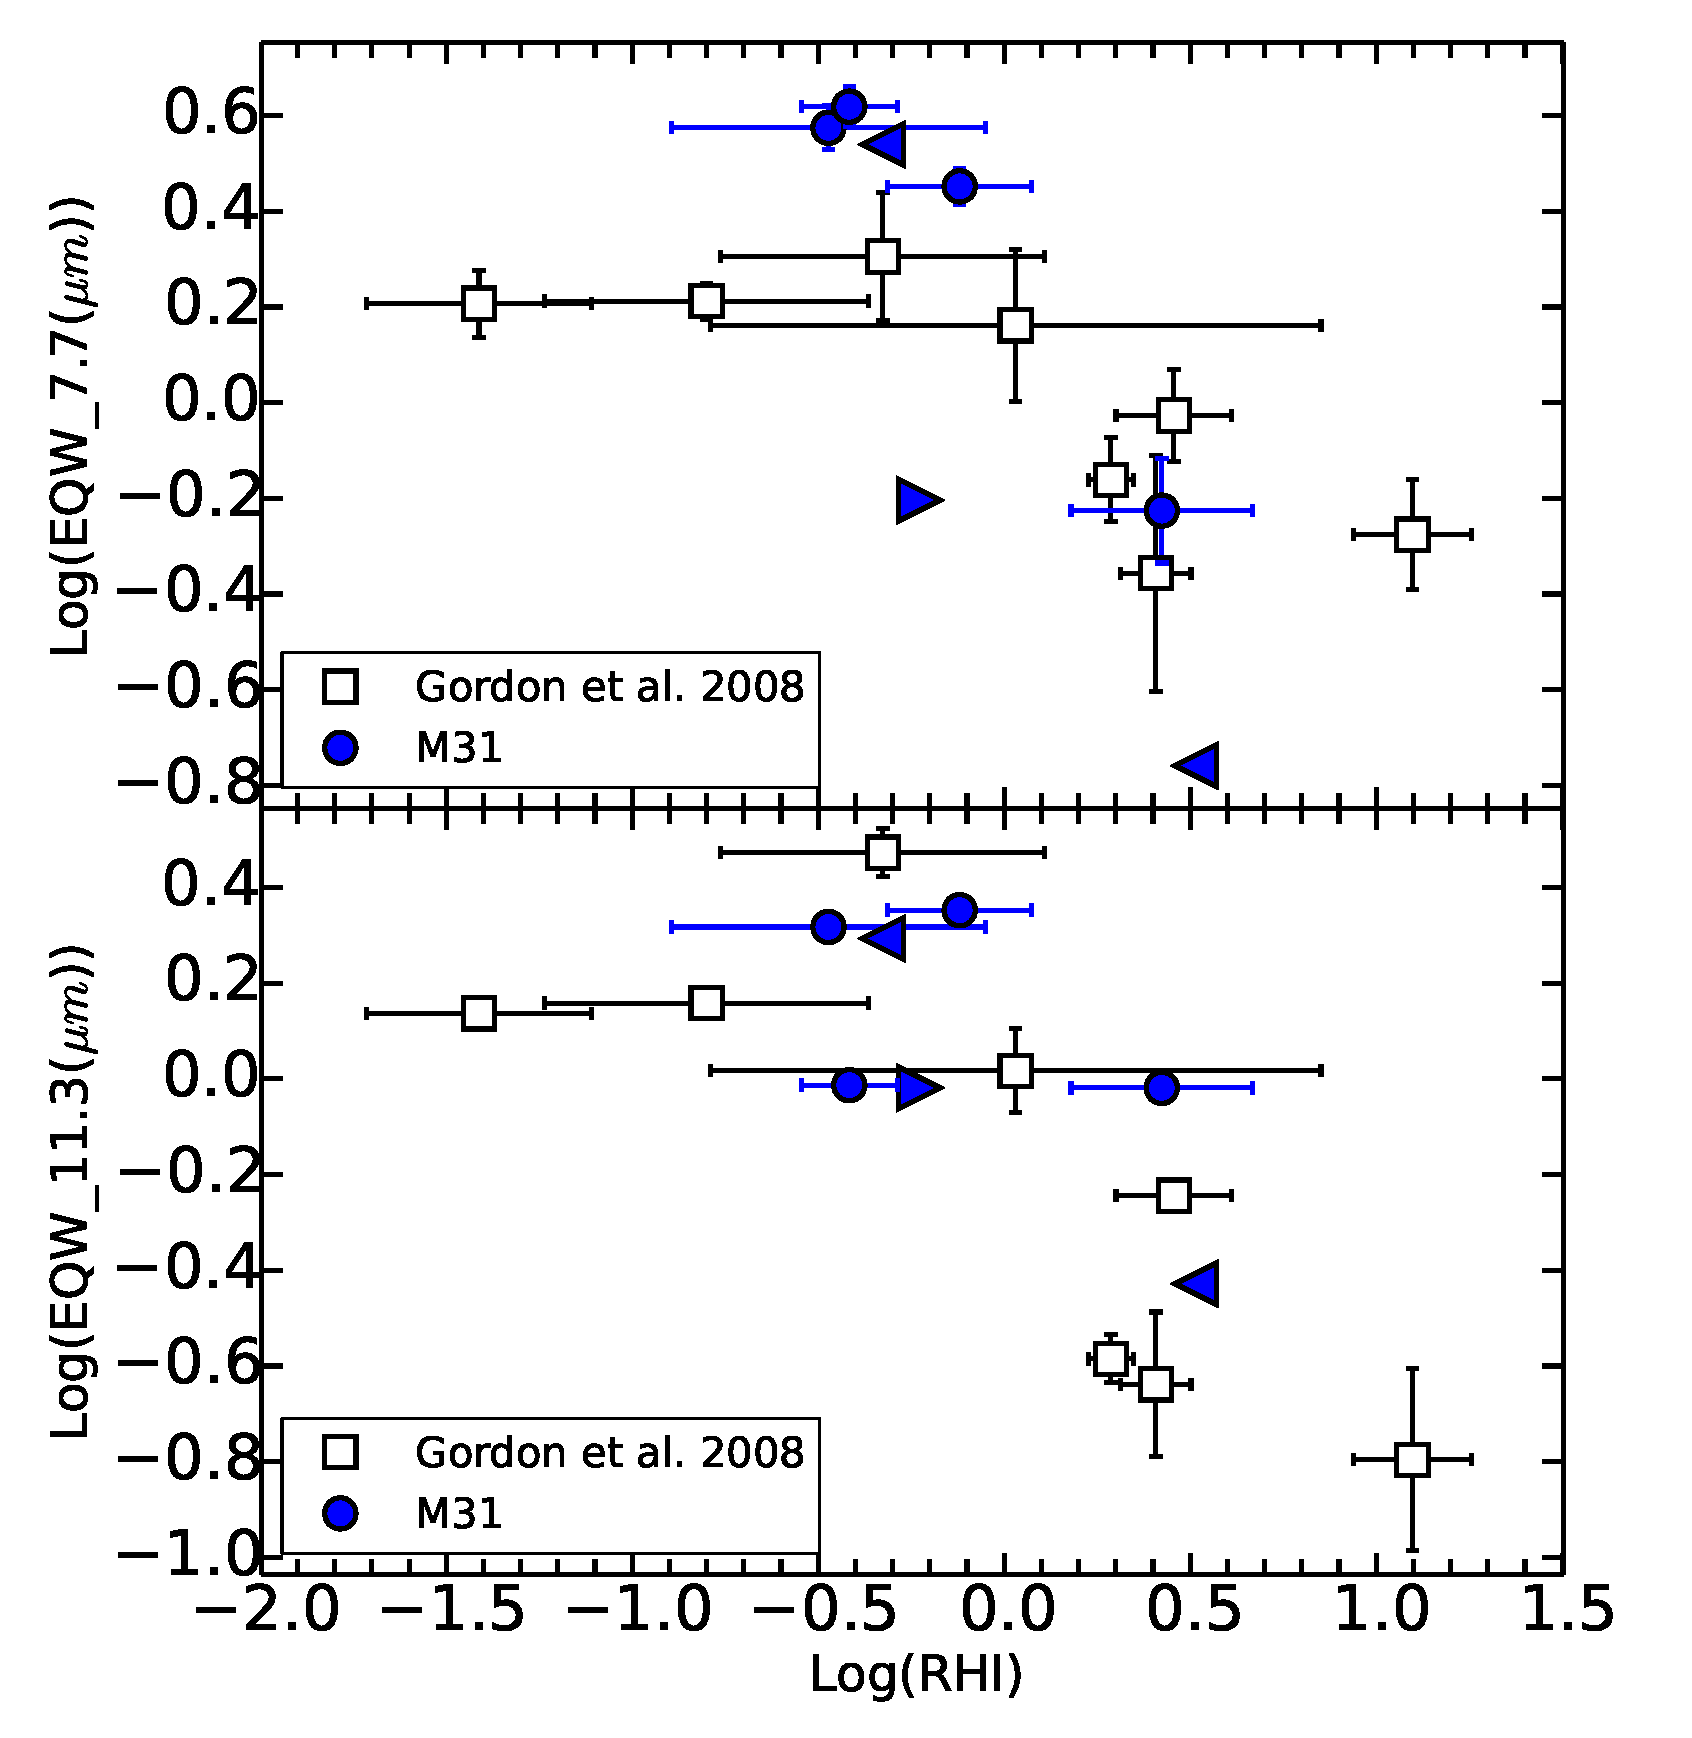
\includegraphics[scale=0.30]{./Gordvsmy.eps}
\caption{Equivalent widths of the normalized 7.7~$\mu$m PAH feature (top panel) and 11.3~$\mu$m PAH feature (bottom panel) versus 
radiation hardness index (RHI) for the M31 sample. Open squares represent the data from M101 by \citet{Gordon:2008lr}. 
The normalization was done by dividing each EQW by the weighted average over all regions in the respective samples. Triangles represent upper and lower limits.}
\label{gordII}
\end{figure}


As mentioned in the introduction, PAH equivalent widths tend to show an inverse correlation with radiation hardness. 
The equivalent widths of the M31 PAH features are compared with RHI in Figures~\ref{englII} and \ref{gordII}.
For reference, we also show the starburst sample of \citet{Engelbracht_2008}, which includes 66 nearby ($2<d<250$~Mpc)
star-bursting or star-forming galaxies selected to cover a wide range in metallicity ($7.1<12+\log{\rm[O/H]}<8.9$),
and the seven H~{\sc ii} regions in M101 observed by \citet{Gordon:2008lr}, which have $8.1<12+\log{\rm[O/H]}<8.8$.
To make a direct comparison with the M101 sample, we normalized the M31 EQWs in Figure~\ref{gordII} using the same procedure
as \citet{Gordon:2008lr}, dividing each EQW by the  weighted average over all regions in the respective samples. 
The equivalent widths seem to be decreasing with increasing radiation hardness, consistent with previous results. 
This also helps to confirm that the PAH emission in M31 is not unusual. 


\subsection{PAH equivalent widths versus metallicity}
\label{sect:eqw_met}

Many studies based on ISO and {\em Spitzer} observations have reported that PAH intensity decreases with decreasing metallicity \citep{Calzetti:2010fk}. 
In addition, these studies also report a sudden drop of EQWs of PAHs around $12+\log{\rm (O/H)} \approx 8.1$. 
This has been observed amongst different galaxies \citep{Engelbracht_2008} as well as within a single galaxy \citep{Gordon:2008lr}. 

Here we investigate the relation between the PAH features and the metallicity for the M31 regions in this paper. 
As a source of metallicity measurements, we used the work of \citet{Sanders_2011} who measured spectroscopic metallicities for
more than 250 H~{\sc ii} regions using strong line diagnostics.\footnote{\citet{Sanders_2011} considered several different
calibrations for abundance diagnostics. We use the results from the method they denote ``N06 N2''  \citep{Nagao2006} because
that method has the largest sample size.} Except for regions 5 and 8, all of our mapped regions contain an  H~{\sc ii} region measured by
 \citet{Sanders_2011}, and we give the corresponding metallicities in Table~\ref{regions}.
 For regions 5 and 8 we adopted metallicities from the radial metallicity profile of M31 given by
 \citet{Sanders_2011}. It is well known that there are systematic differences between different 
 methods used to measure metallicities, and those in the sample of \citet{Engelbracht_2008} 
 were obtained by the direct electron temperature method  \citep{Skillman1998}.
\citet{Mitchel2014} calculated the offset between direct and strong-line measurements for M31 H~{\sc ii} regions to be 
$0.35\pm0.10$. In Figure \ref{metalicityVseqw} we have corrected for this offset  by subtracting 0.35 from our metallicities. 

%SPW:In the discussion of Fig 13, I think it's worth mentioning that no trend is seen, but there are relatively few data points.
\begin{figure}
\centering
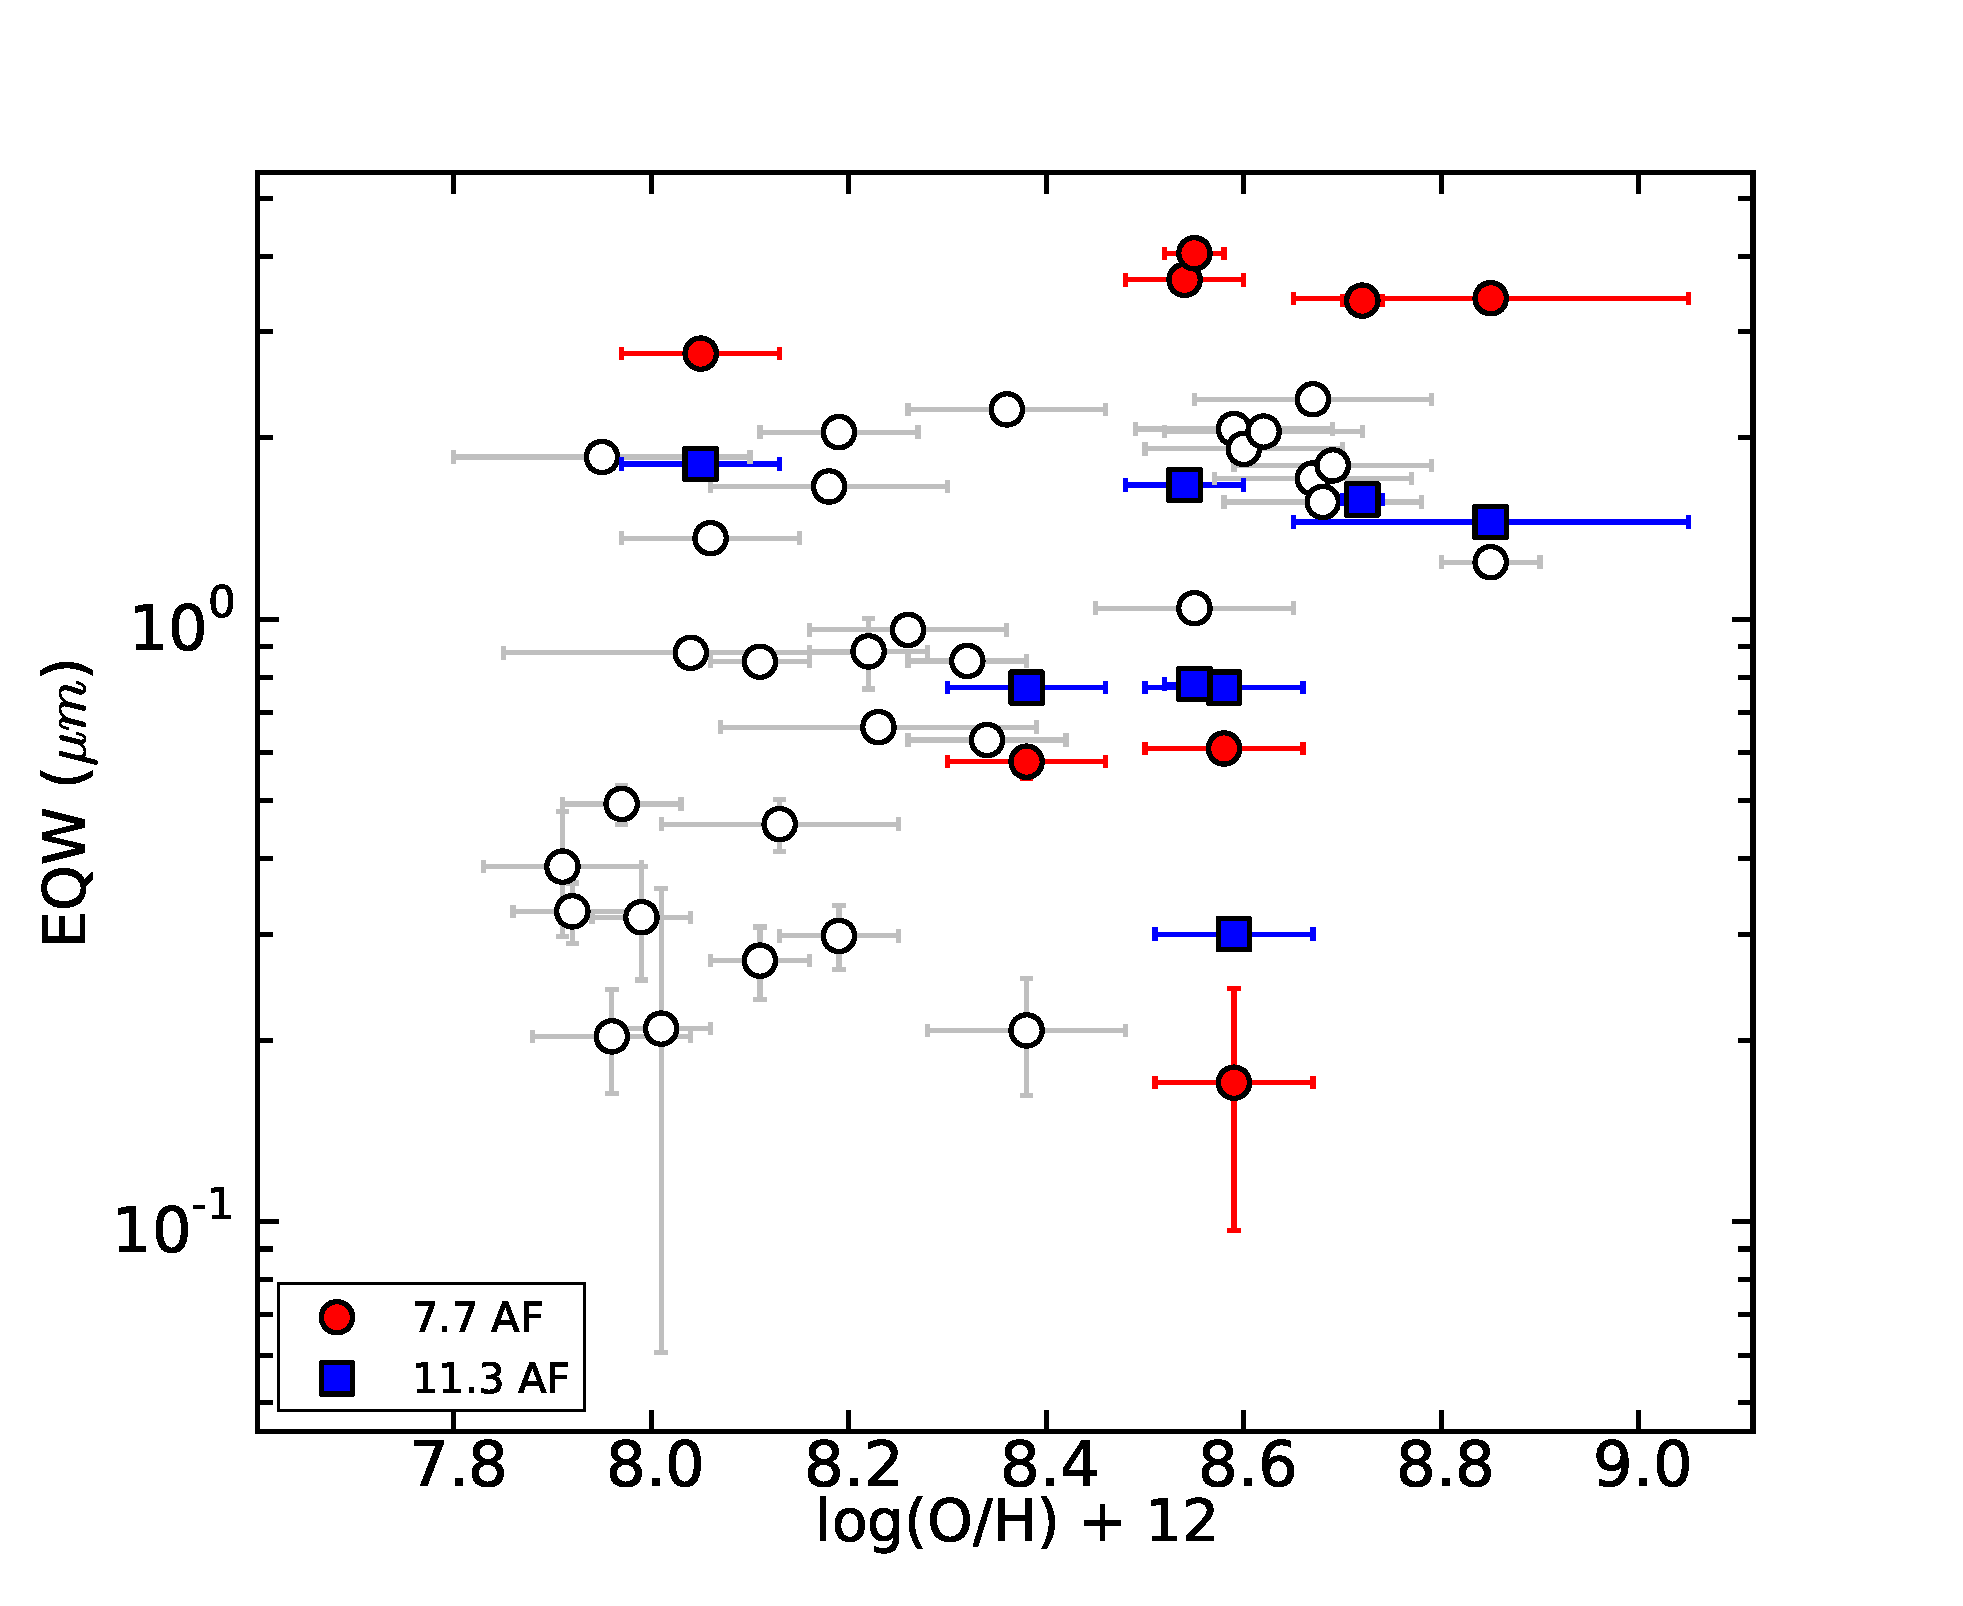
\includegraphics[scale=0.27]{./oxyvseqw.eps}
\caption{ PAH equivalent widths versus metallicity. EQWs of the 7.7~$\mu$m feature of the starburst sample from \citet{Engelbracht_2008} are plotted in open circles.}
\label{metalicityVseqw}
\end{figure}

Figure \ref{metalicityVseqw} shows the normalized EQWs of the PAH features  versus the metallicity for our sample and the starburst 
galaxies of \citet{Engelbracht_2008}. The scatter in our sample is large, but the 	
equivalent widths of the 7.7 and 11.3~$\mu$m features are not inconsistent with those of \citet{Engelbracht_2008}. 
However, we do not have enough data from low-metallicity regions in M31 to observe the expected decrease of EQWs of PAH with the decreasing 
metallicity.  There do seem to be some outliers which can plausibly be due to the uncertainties  and the offset between different methods of calculating the metallicity.  
%SPW: Sec 4.2 par 4: while there's no metallicity dependence, 1 region has very low PAH.    Any idea why?  Is it just stellar light contamination, or is something fundamental happening?

\subsection{Dust properties of the nucleus}
\label{sect:nucleus}

\begin{figure}
\centering
\caption{Here is where we show the PAHFIT analysis of the nucleus spectrum.}
\label{fig:nuc_pahfit}
\end{figure}


The extracted IRS spectrum of the M31 nuclear region (Figure~\ref{fig:nuc_pahfit})
looks different from most of the other spectra, with
a blue continuum, PAH features weak or absent at 6--8~$\mu$m  but detectable at 11.3~$\mu$m.
{\bf NEED some further discussion of the nuclear spectrum in general here.}
Figure \ref{nuc11} (top) shows the integrated intensity map of 11.3~$\mu$m emission around the nucleus. The majority of the 11.3~$\mu$m 
emission is from a region north of the nucleus and not from the nucleus itself. 
On the other hand the centre shows no PAH emission,  but it does have silicate emission around 9.7~$\mu$m, 
which comes only from the nucleus and is not present in the North spectrum 
(see Figure \ref{nuc11} (bottom), a continuum-subtracted image which shows the 9--11~$\mu$m integrated emission).
Both the 11.3~$\mu$m  and silicate emission sources are consistent with being unresolved point sources.
We extracted spectra from the centre and the North region using a $9\arcsec \times 9\arcsec$ 
square aperture as shown in Figure \ref{nuc11}. 


\begin{figure}
\centering
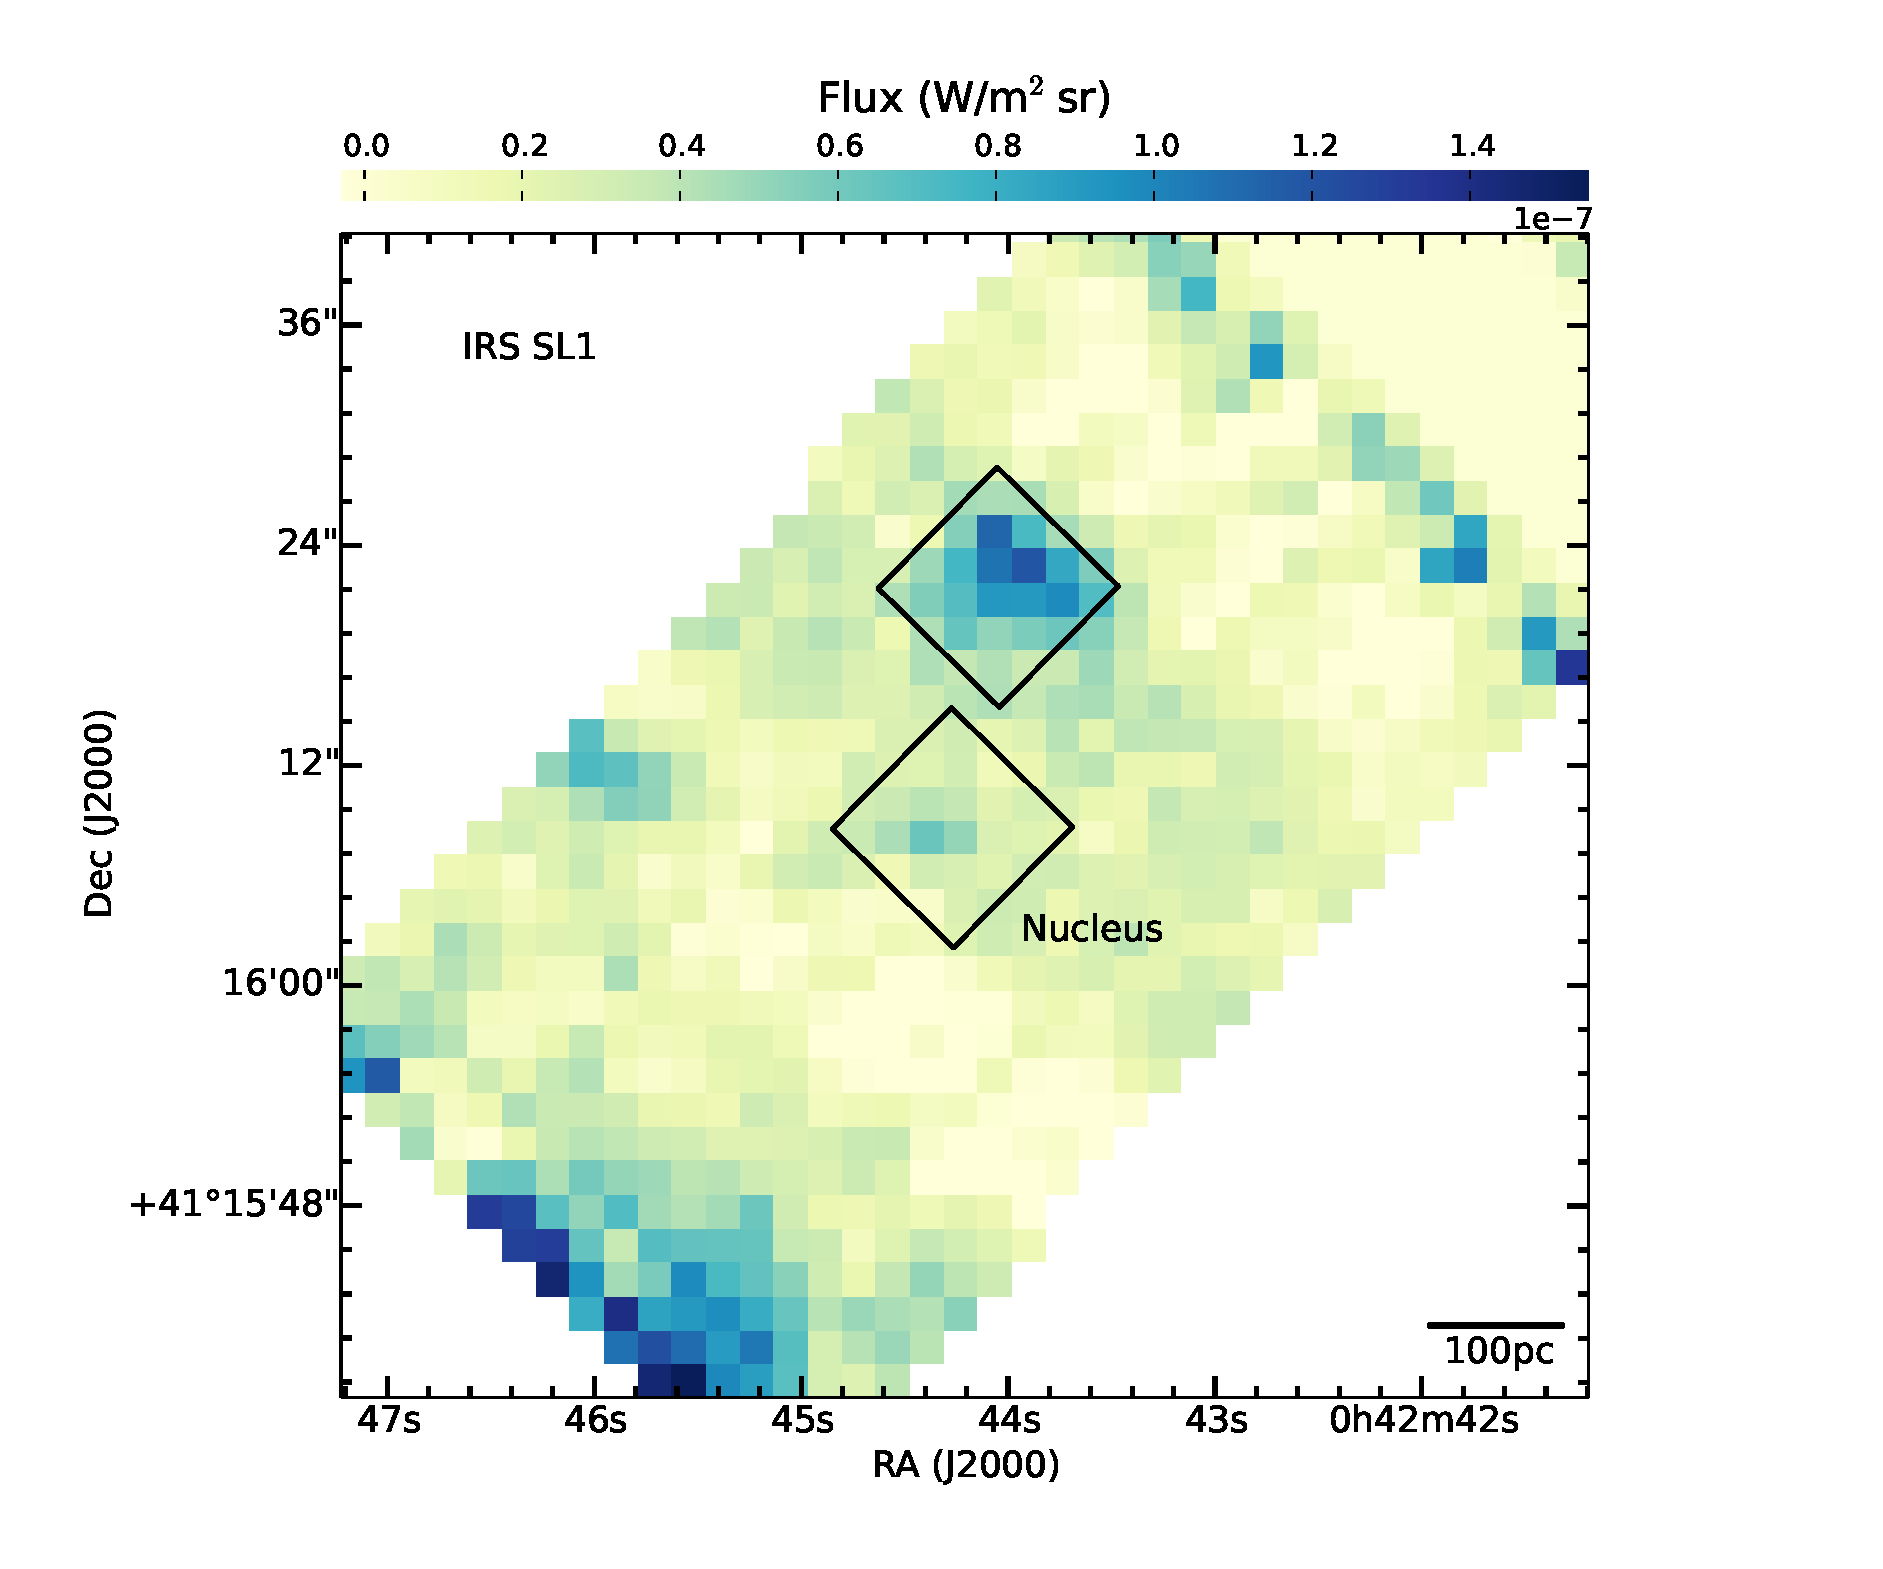
\includegraphics[width = 8 cm]{./nuc11_3.eps}
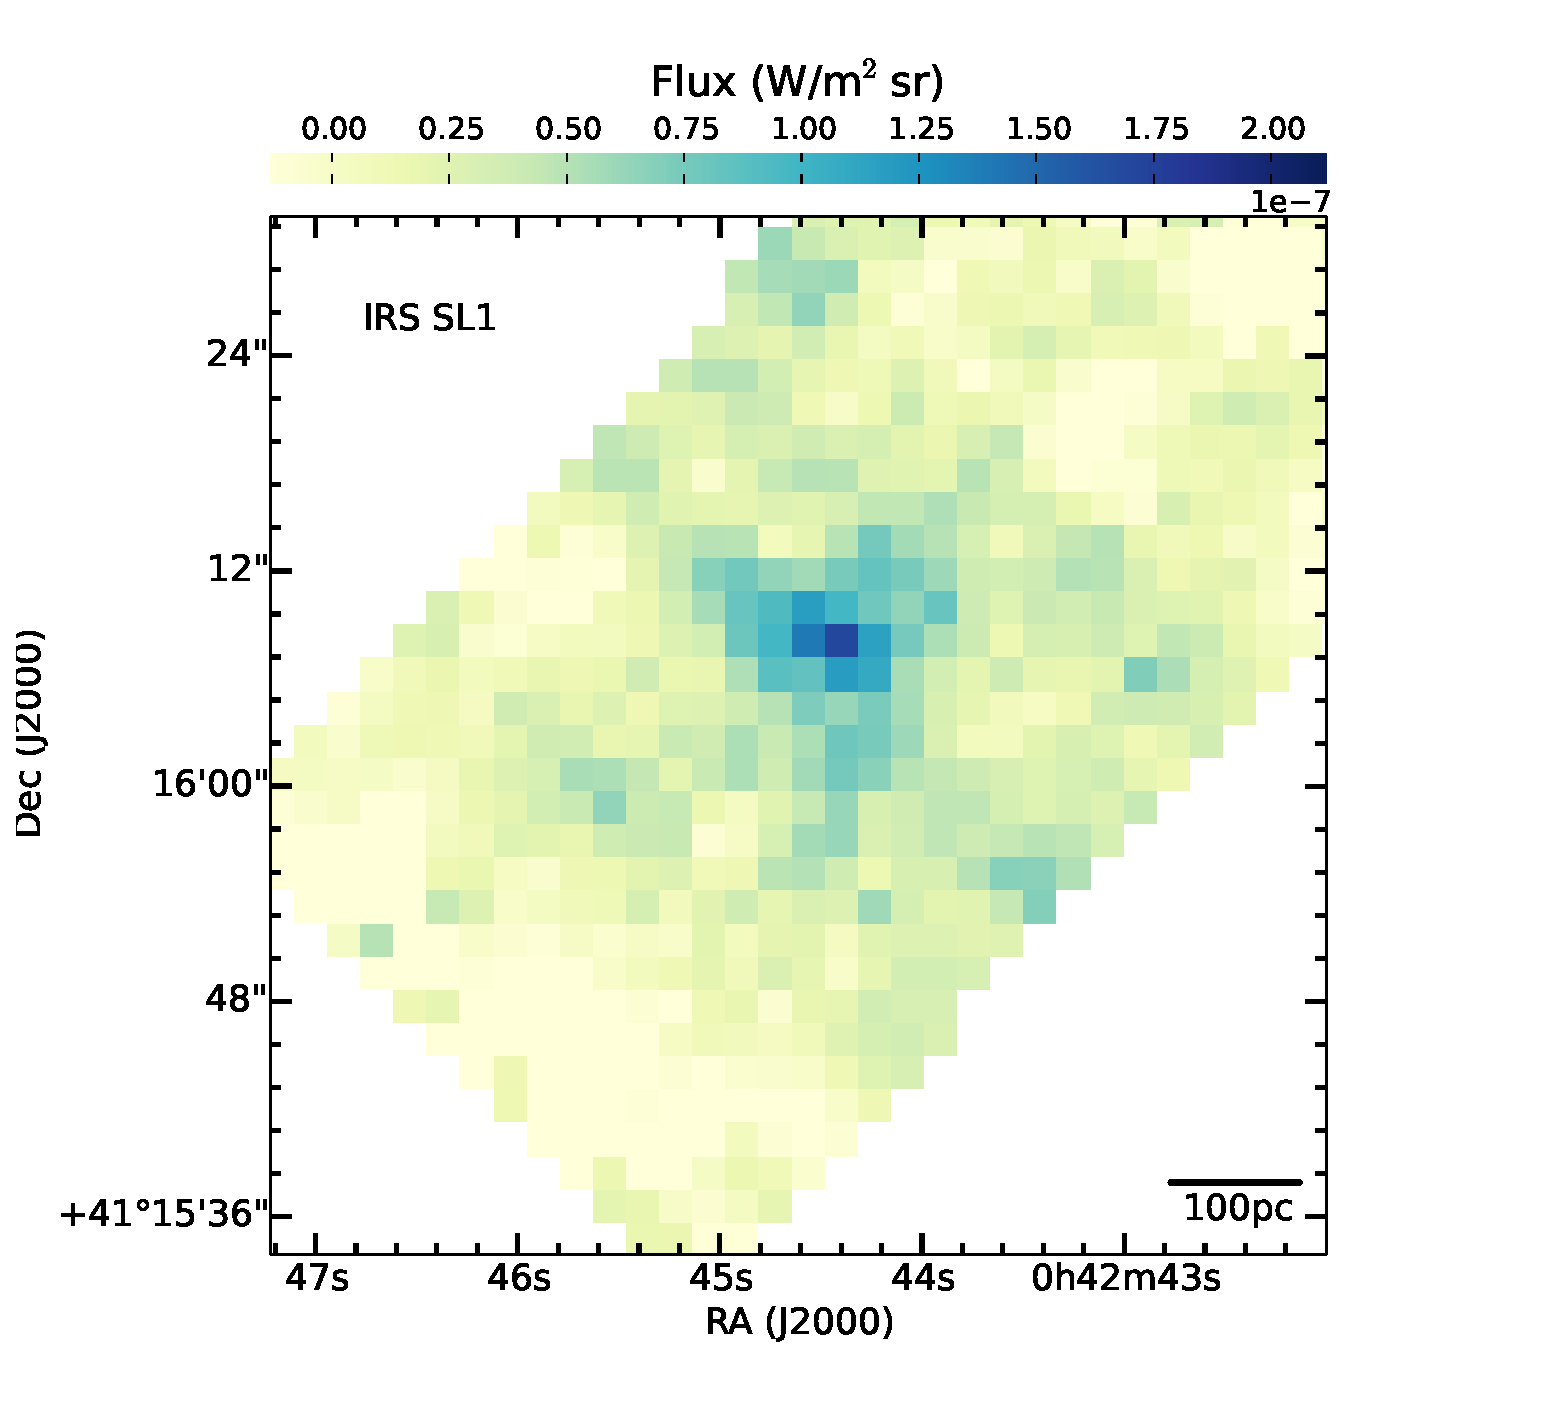
\includegraphics[scale = 0.3]{./NUCsilicate.eps}
\caption{(Top): Intensity variation of 11.3~$\mu$m emission around the nucleus of M31. 
Two black boxes are the apertures (centre and north region) used to extract spectra in Figure \ref{smithspec}. 
The centre of the nucleus is at R.A. $00^{\rm h}42^{\rm m}44\fs35$, Dec. $+41\degr16\arcmin08\farcs5$ \citep{NucleusREF}.
(Bottom:) Integrated strength of the silicate emission (from 9 to 11~$\mu$m) near the M31 nucleus.}
\label{nuc11}
\end{figure}




%
%I guess the nuclear spectrum is in your Figure 15 - why did you not try to fit it with PAHFIT too?  It looks to me like it has a weak 20um silicate bump too.
% Why not include the nuclear region in Tables 2,3&4?  I did not understand the reason for leaving it off.  Also please add the limit for the [Ne V] detection - it might still be a useful ratio with [Ne II] and the PAH lines.  It looked to me like there was some hint of the H2 12.28um line in some regions.... maybe add that limit too, though I was surprised

\begin{figure*}
\centering
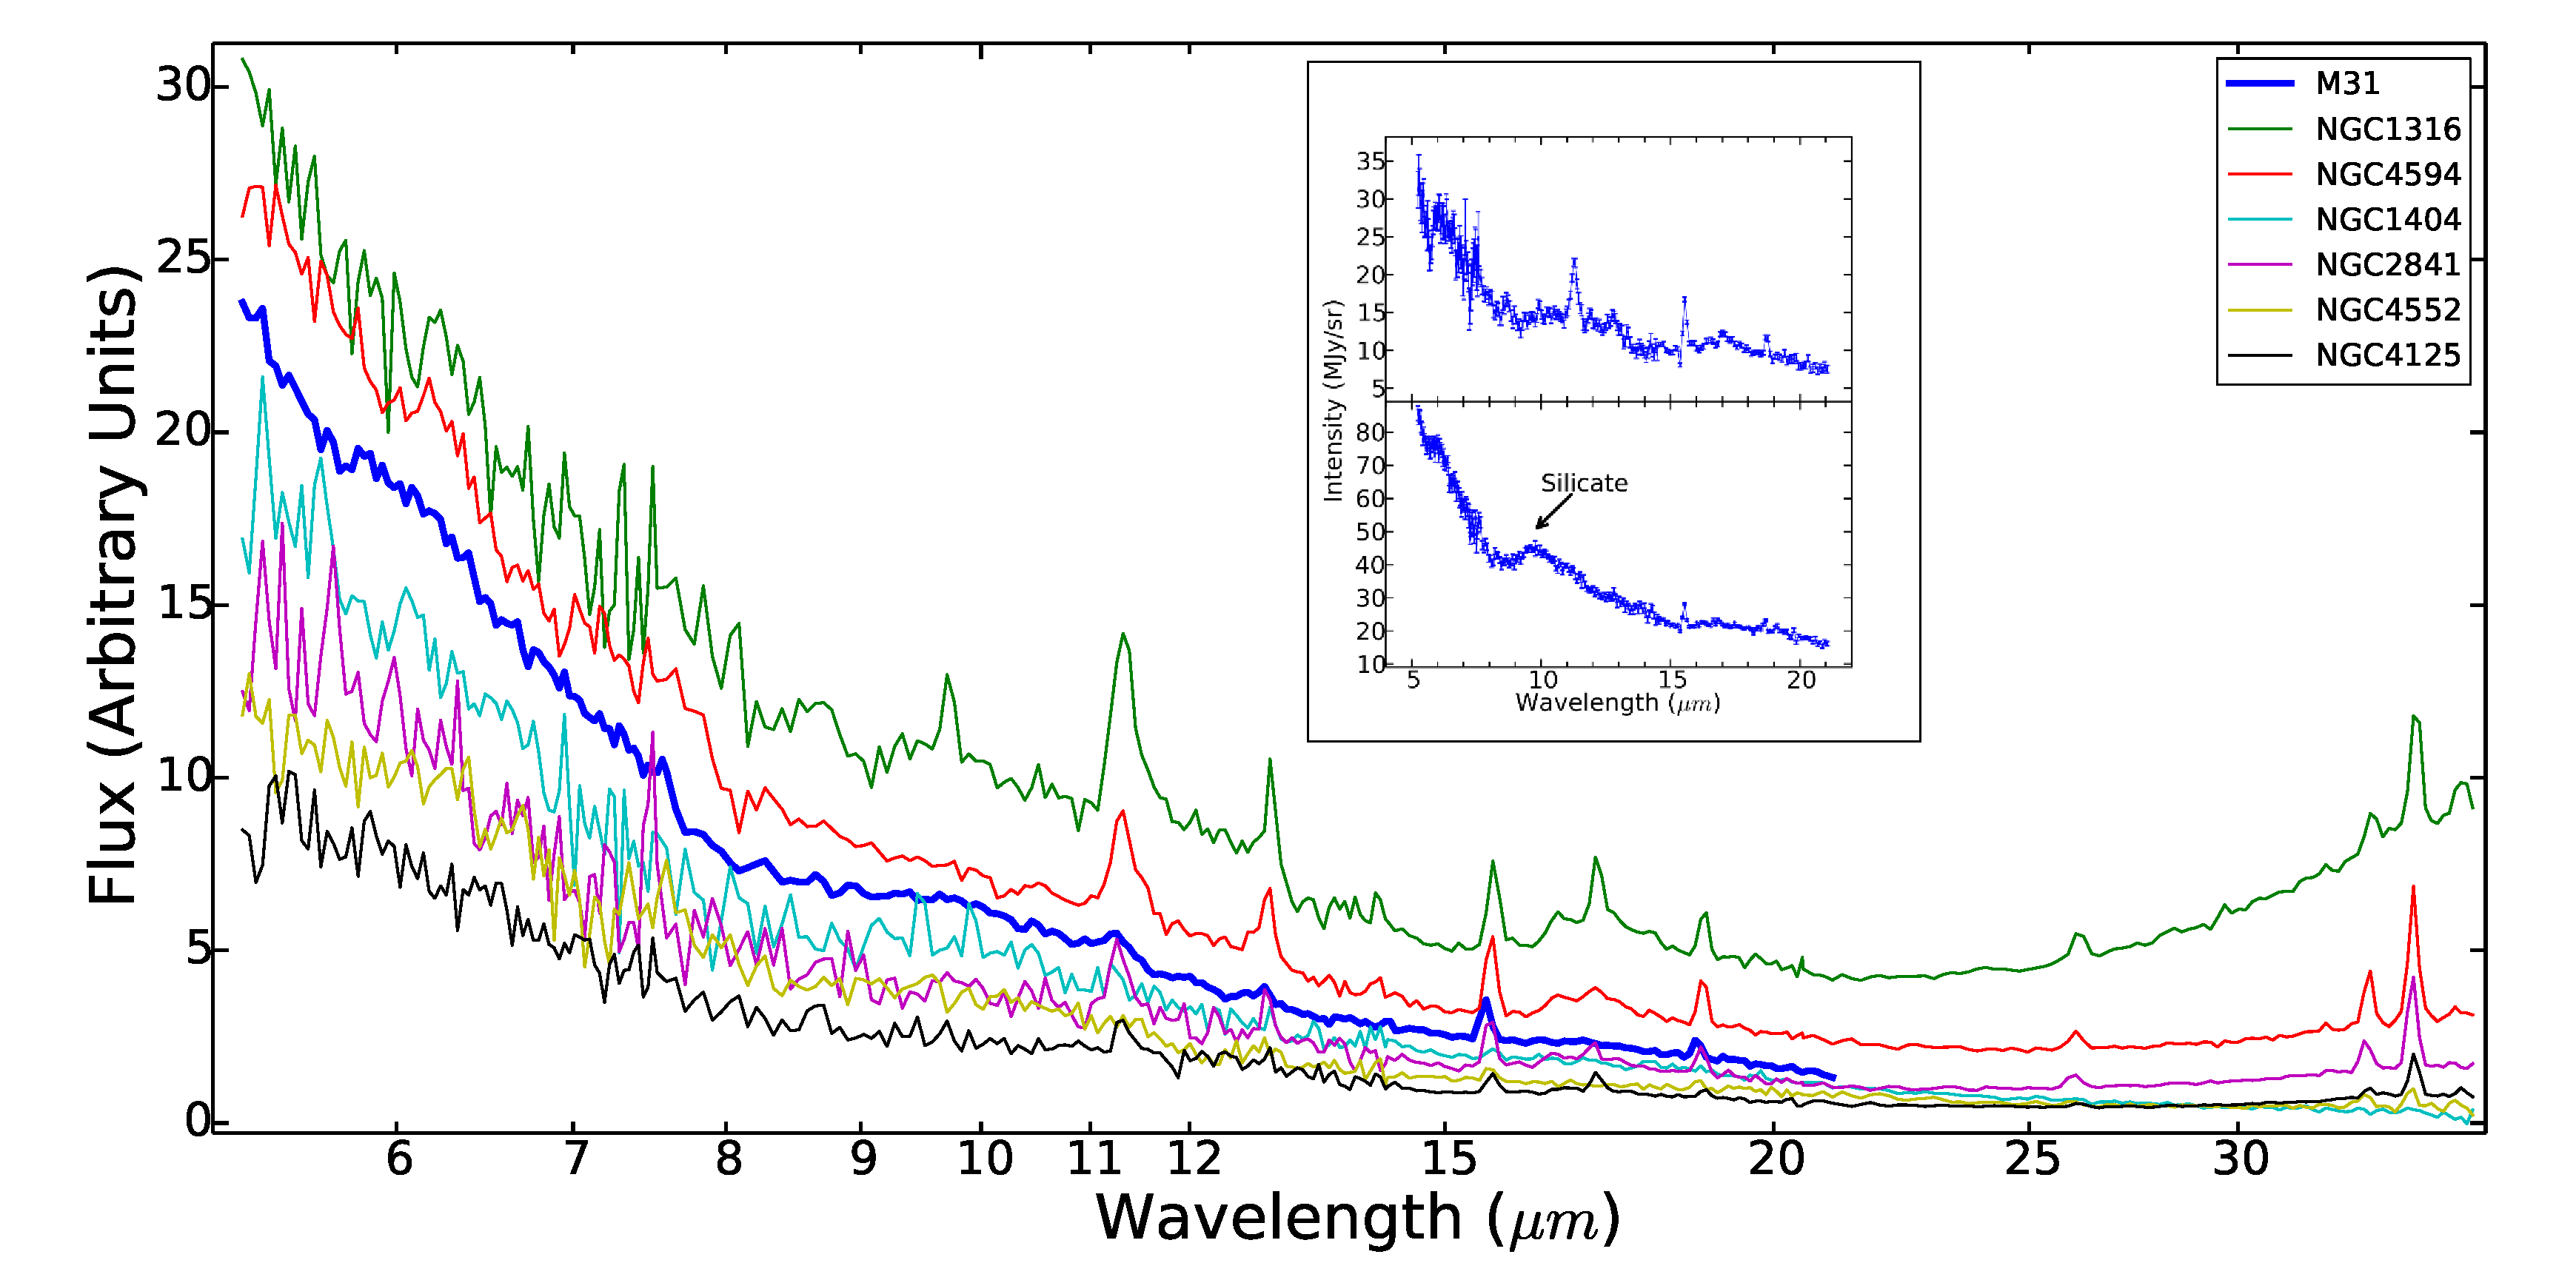
\includegraphics[height = 8 cm]{./SINGSspec.eps}
\caption{Mid-infrared spectrum of the nucleus of M31 (blue) over-plotted with spectra extracted close to the nuclei of 6 nearby galaxies which have 
AGN activity \citep{Smith:2007lr}. NGC 4552, NGC 1404 and NGC 4125 are elliptical galaxies and NGC 4594 and NGC 2841 are spiral galaxies. 
NGC 1316 is a lenticular galaxy. The inset shows the spectra extracted from the centre region of the M31 nucleus (bottom) and from the north region (top) 
shown in Figure \ref{nuc11}.}
\label{smithspec}
\end{figure*}

The mid-infrared spectra of the nucleus from both {\em Spitzer} and ISOCAM (Figure~\ref{ISOnIRS}) show similar characteristics: a blue
continuum, PAH features weak or absent at 6--8~$\mu$m  but detectable at 11.3~$\mu$m, and detectable atomic fine structure lines.
Comparing the M31 nuclear spectrum with the nuclear spectra from the SINGS sample given by \citet{Smith:2007lr}, we found
six other galaxies with similar spectral shapes, including three elliptical galaxies, two spirals, and a lenticular.%
\footnote{The IRS spectra for the SINGS galaxies were extracted over areas ranging from 2 to 8 kpc$^2$, whereas the M31
nucleus spectrum covers a much smaller area (0.02~kpc$^2$).}
The SINGS papers \citep{kennicutt03,Smith:2007lr, moustakas2010} are in some disagreement over the
exact nuclear spectral types of these six galaxies. All are classified as some form of low-luminosity AGN
such as Seyfert or LINER \citep[luminous AGNs were intentionally omitted from the SINGS sample][]{kennicutt03}, but they are
by no means the only LLAGN in the SINGS sample.
In contrast with the nuclear spectrum, the spectrum extracted in the North region (offset by \arcsec from the center;
Figure \ref{smithspec}, inset) shows a strong 11.3~$\mu$m peak 
and no significant emission from 6--8~$\mu$m features. These characteristics are shared by
the M81 nuclear spectrum presented by \citet{Smith2010}, although that spectrum has little stellar continuum and a very strong [Ne {\sc ii}]~12.8~$\mu$m line. 


As discussed by  \citet{Smith:2007lr} and \citet{Smith2010}, inferring the suppression of 6--8~$\mu$m PAH features compared
to the 11.3~$\mu$m feature must be done with caution, since the 6--8~$\mu$m features are more susceptible to dilution by the stellar
continuum. Such suppression could have several causes: destruction of small or charged PAH molecules by an AGN,
or weak ultraviolet continuum indicating lack of star formation \citep{Smith:2007lr}. In the latter case, the AGN is not the cause of
the suppressed  6--8~$\mu$m features, but rather is only detected when the nuclear star formation rate is low.
An implication of low star formation in the centre of M31 is consistent
with previous work: although \citet{Melchior2013} found a significant amount of cold gas in the centre of the galaxy, this gas does not
appear to be associated with current star formation. In modelling the far-infrared spectral energy distribution, \cite{Groves2012} found that  
the old stellar population in the M31 bulge is sufficient  to heat the observed dust; no young stellar population is needed.


Examining the spatial distribution of the mid-infrared emission in the M31 nuclear region provides additional clues
to the nature of the emitting sources. Figure~\ref{nuc11} shows that most of the 11.3~$\mu$m comes from a region to the
north of the nucleus, while the silicate emission (Figure~\ref{nuc11},  bottom) is centred on the nucleus itself.  Figure \ref{smithspec}
compares the spectra extracted from these two regions. Silicate emission is not very common in
integrated spectra of galaxies \citep{Spoon2007} but is seen in luminous quasar spectra \citep{Hill14} and, as mentioned above, in the
spectrum of the M81 nucleus. We computed the linear slope parameter  defined by \citet{Smith2010},
$\gamma810 =[F_{\nu}(10\mu{\rm m}) -F_{\nu}(8\mu{\rm m})]/2F_{\nu}(9\mu{\rm m}) $, for the M31 nucleus and
found $\gamma810 =-0.08\pm 0.06$.  This is 
%HAS: It might be useful to tabulate the masses of the black holes in each of the 6 comparison galaxies, to see whether spectral similarities (or differences) can be attributed to the quiescent AGN, as you suggest, of whether circumnuclear star formation or other things might play some role.


Does detection of silicate emission in the M31 nuclear spectrum imply the detection of an active nucleus?
In the unified model of AGNs, an obscuring torus viewed face-on would be expected to show silicate emission
\citep{AGNtypes1995, AGNref}; however such a view would also be expected to show forbidden atomic lines such as [Ne~{\sc v}] and [S~{\sc iv}],
not seen in the M31 spectrum. Alternatively, \citet{Mason2012} explained that low-luminosity AGNs cannot 
host a Seyfert-like obscuring torus because of their optically thin dust and low dust-to-gas ratio, but can show
the silicate emission that originates in the optically thin hot dust around the torus.  The first detection of such silicate emission was 
reported by \citet{Sturm2005} from the low-ionization nuclear emission-line region (LINER) galaxy NGC~3998, and 
\citealt{Mason2012}  observed that this 9.7~$\mu$m silicate emission is present in many LLAGNs. 
We computed the bolometric luminosity of the M31 nucleus  to be (**value goes here**) erg~s$^{-1}$ using the 12~$\mu$m flux 
and the method described in \citet{luminosity}. This value is close to that of other LLAGNs (**and consistent with the X--ray value?**)
